\section{طراحی و شبیه‌سازی کنترل‌کننده برای کانال رول-پیچ}
\label{roll_pitch_lqidg_section_simulation}
در بخش
\ref{quadchanell_roll_pitch}
شبیه‌سازی کانال رول-پیچ استند چهارپره انجام شد. در این بخش به بررسی عملکرد چهارپره در حضور کنترل‌کننده \lr{LQIDG} پرداخته می‌شود. کنترل‌کننده \lr{LQIDG}  در بخش
\ref{LQIDG}
بررسی شده است.
 در شبیه‌سازی برای بهینه‌سازی ضرایب وزنی \lr{LQIDG} از روش بهینه‌سازی
\lr{TCACS} \cite{Karimi2010}
استفاده شده‌است.
تابع هزینه \lr{TCACS} به‌صورت
\lr{ITSE}
در نظر گرفته شده‌است. ضرایب وزنی خروجی بهینه‌سازی در پایین آورده شده‌است. برای طراحی کنترل‌کننده
\lr{LQIDG}
ضرایب وزنی
$R_1$
و
$R_2$
برای کانال‌های مختلف یکی فرض شده‌است.
\begin{equation}
	\begin{split}
		\boldsymbol{Q_{a_{LQIDG_{roll}}}} &= \begin{bmatrix}
			585.9 &0& 0& 0\\
			0 &  31.1 & 0 &0 \\
			0 & 0 & 83.8 & 0\\
			0 & 0 & 0 & 0
		\end{bmatrix} ,
	\boldsymbol{Q_{a_{LQIDG_{pitch}}}} = \begin{bmatrix}
		546.5 &0& 0& 0\\
		0 &  311.4 & 0 &0 \\
		0 & 0 & 2.22 & 0\\
		0 & 0 & 0 & 0
		\end{bmatrix}\\
	R_{1_{LQDG}} &=  1,\qquad  \qquad \qquad \qquad \quad R_{2_{LQDG}} =  7.7422
	\end{split}
\end{equation}

در گام بعد، با حل معادله
(\ref{coupled_riccatti_LQIDG})
(برای سادگی ماتریس‌های وزنی $\boldsymbol{\dot{Q}_{a_2}}$ و $\boldsymbol{\dot{Q}_{a_1}}$مساوی در نظر گرفته شده‌است)
ماتریس
$\boldsymbol{\dot{K}_1}$
به‌صورت زیر به دست می‌آید.
\begin{equation}
	\boldsymbol{K_{a_{1_{roll}}}} = \begin{bmatrix}
1720.86 & 80.29 & 187.71 & -8.57 \\
80.29 & 20.44 & 8.11 & 0.53 \\
187.77 & 8.11 & 686.56 & -0.02 \\
-8.57 & 0.53 & -0.02 & 9.93 \\
	\end{bmatrix}, \boldsymbol{K_{a_{1_{pitch}}}} \begin{bmatrix}
243.90 & 25.01 & 80.29 & -9.50 \\
25.01 & 7.41 & 7.33 & 0 \\
80.29 & 7.33 & 239.14 & 0 \\
-9.50 & 0 & 0 & 9.50 \\
\end{bmatrix}
\end{equation}
در نهایت فرمان کنترلی بهینه بازیکن اول از رابطه
(\ref{LQIDG_u})
به‌صورت زیر به دست می‌آید.
\begin{equation}
	\begin{split}
		u_{1_{roll}} &= -\begin{bmatrix}
			79.7522 &20.4432 &8.1058 &0.5344 
		\end{bmatrix} \boldsymbol{x_{a_{roll}}} \\
	u_{1_{pitch}} &= -\begin{bmatrix}
		25.0112 &7.40730 &7.3280 &0.0010
	\end{bmatrix} \boldsymbol{x_{a_{pitch}}}
	\end{split}
\end{equation}
%\begin{figure}[H]
%	\centering
%	\begin{subfigure}
%		\centering
%		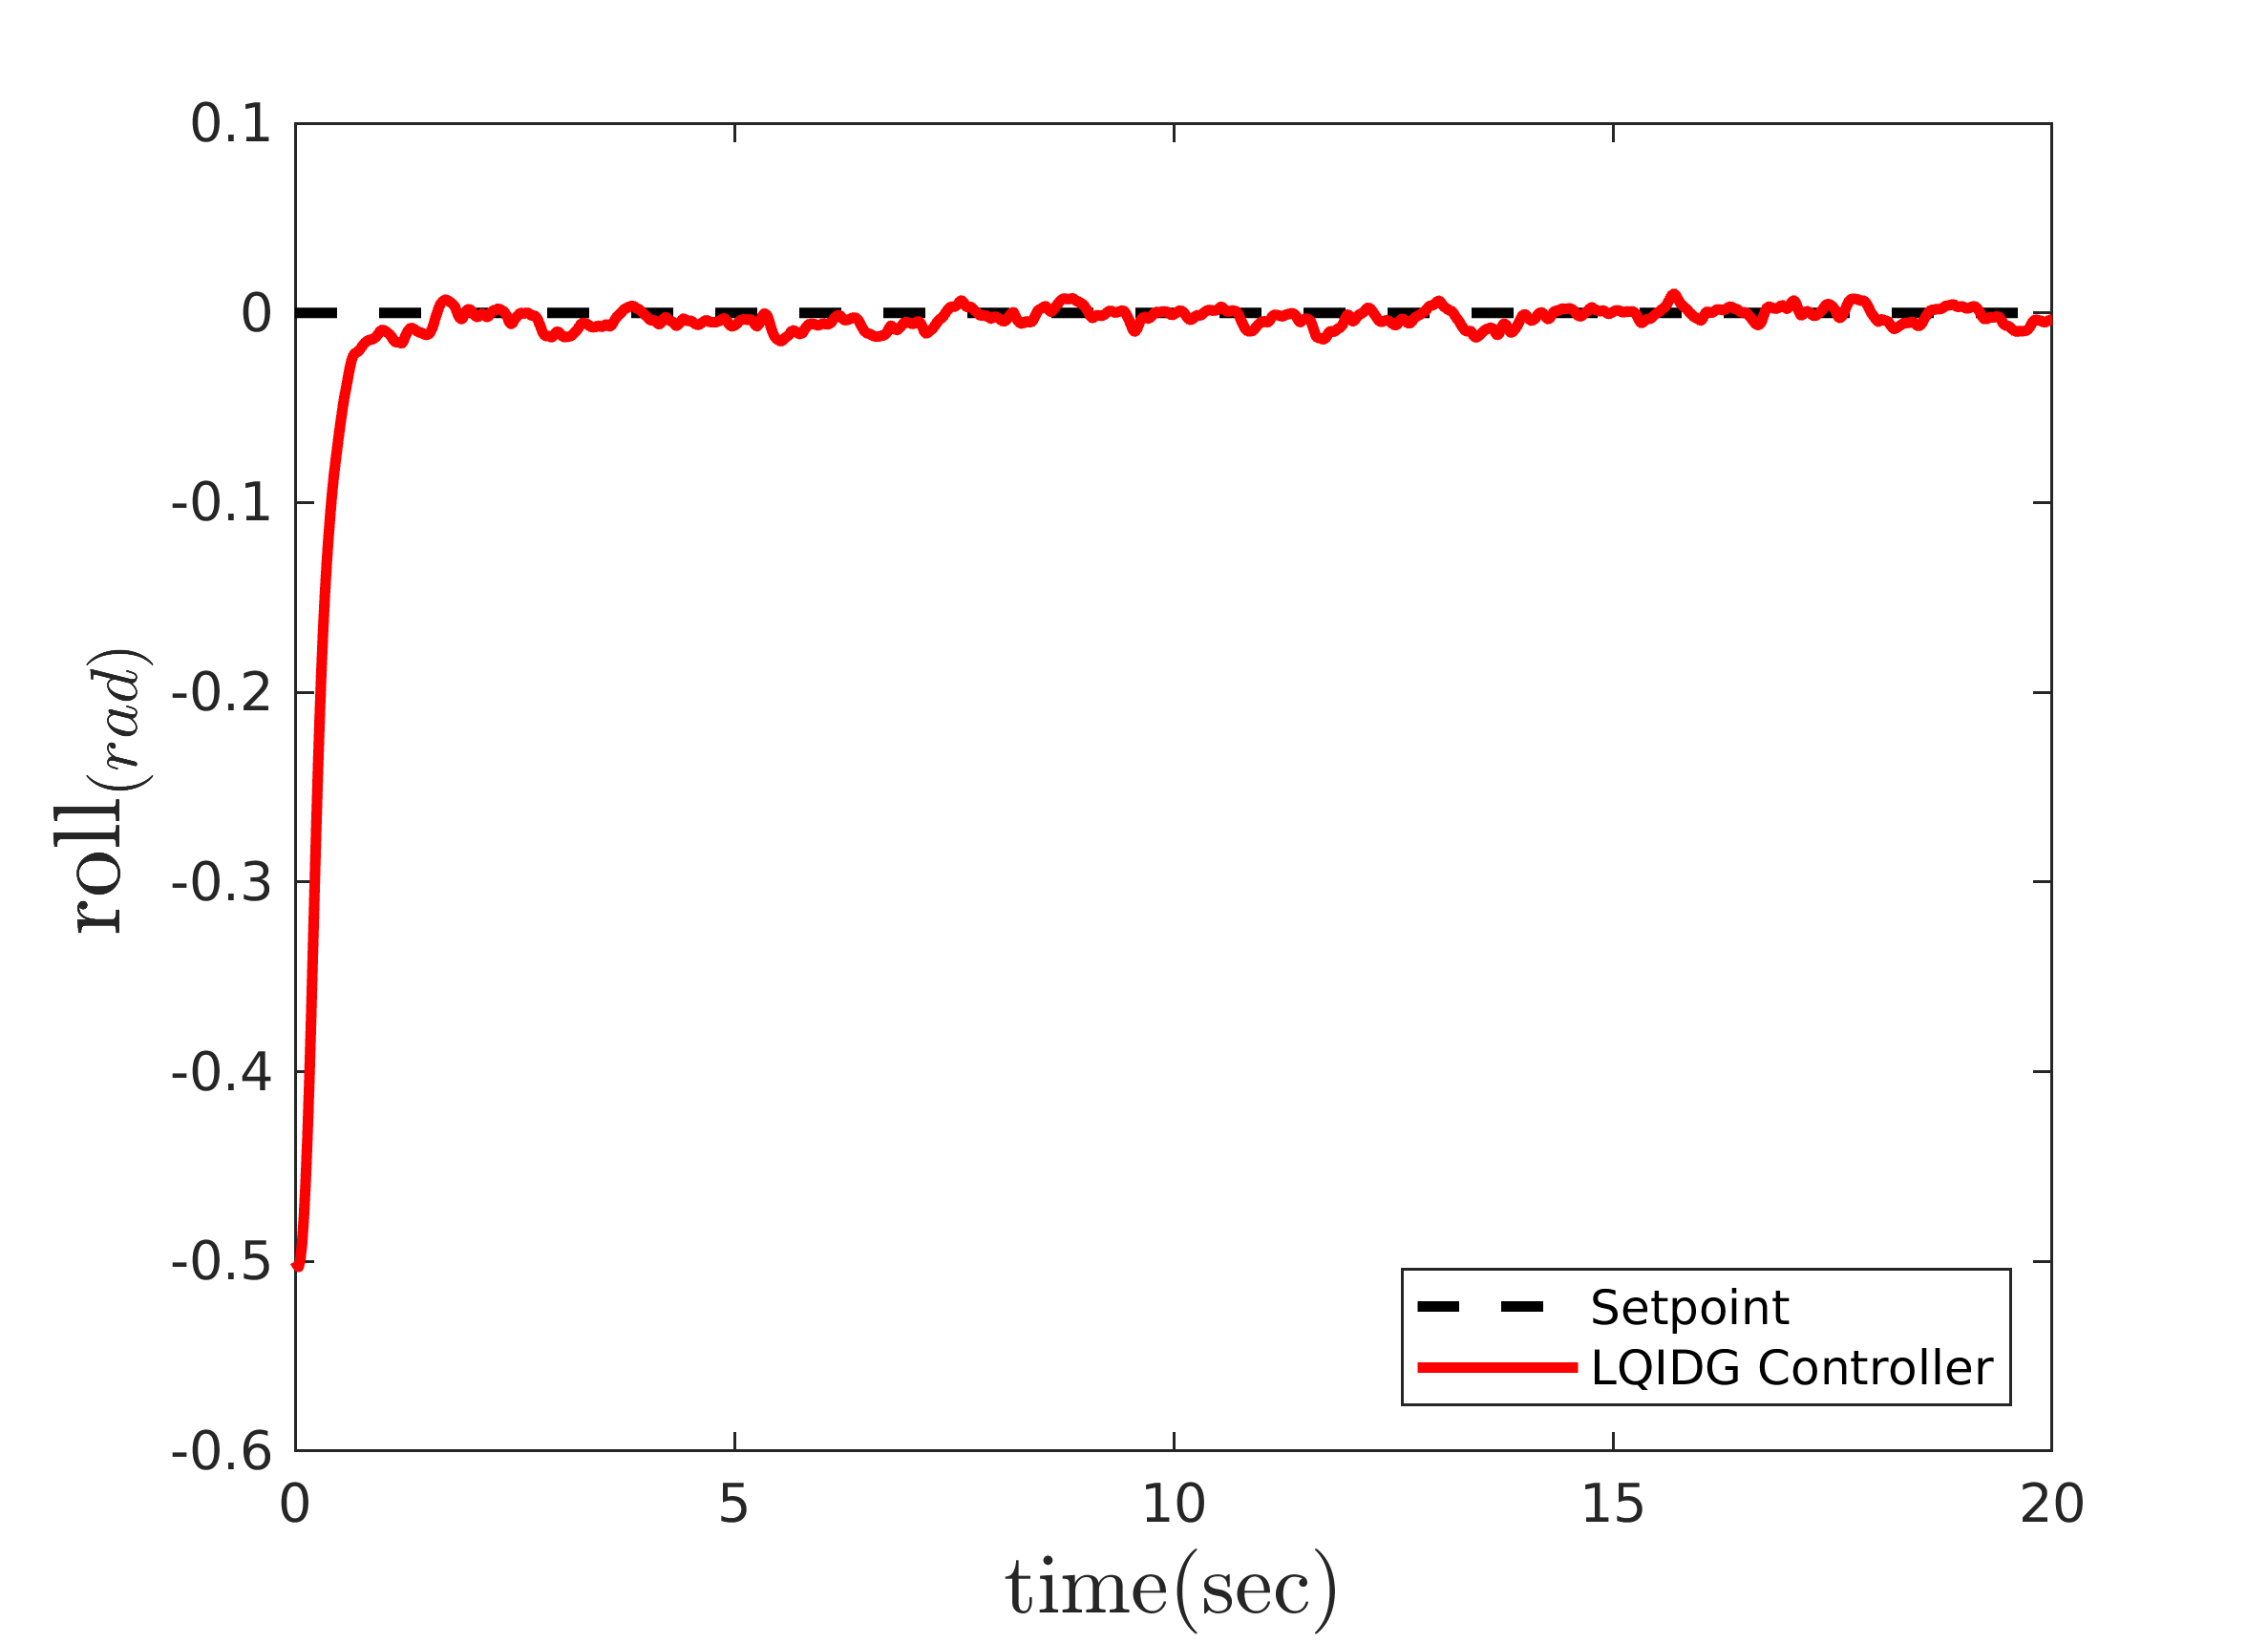
\includegraphics[width=12cm]{../Figures/MIL/LQIDG/Roll_Pitch/lqidg_roll.png}
%		\caption{تغییرات زاویه رول}
%	\end{subfigure}%
%	\begin{subfigure}
%		\centering
%		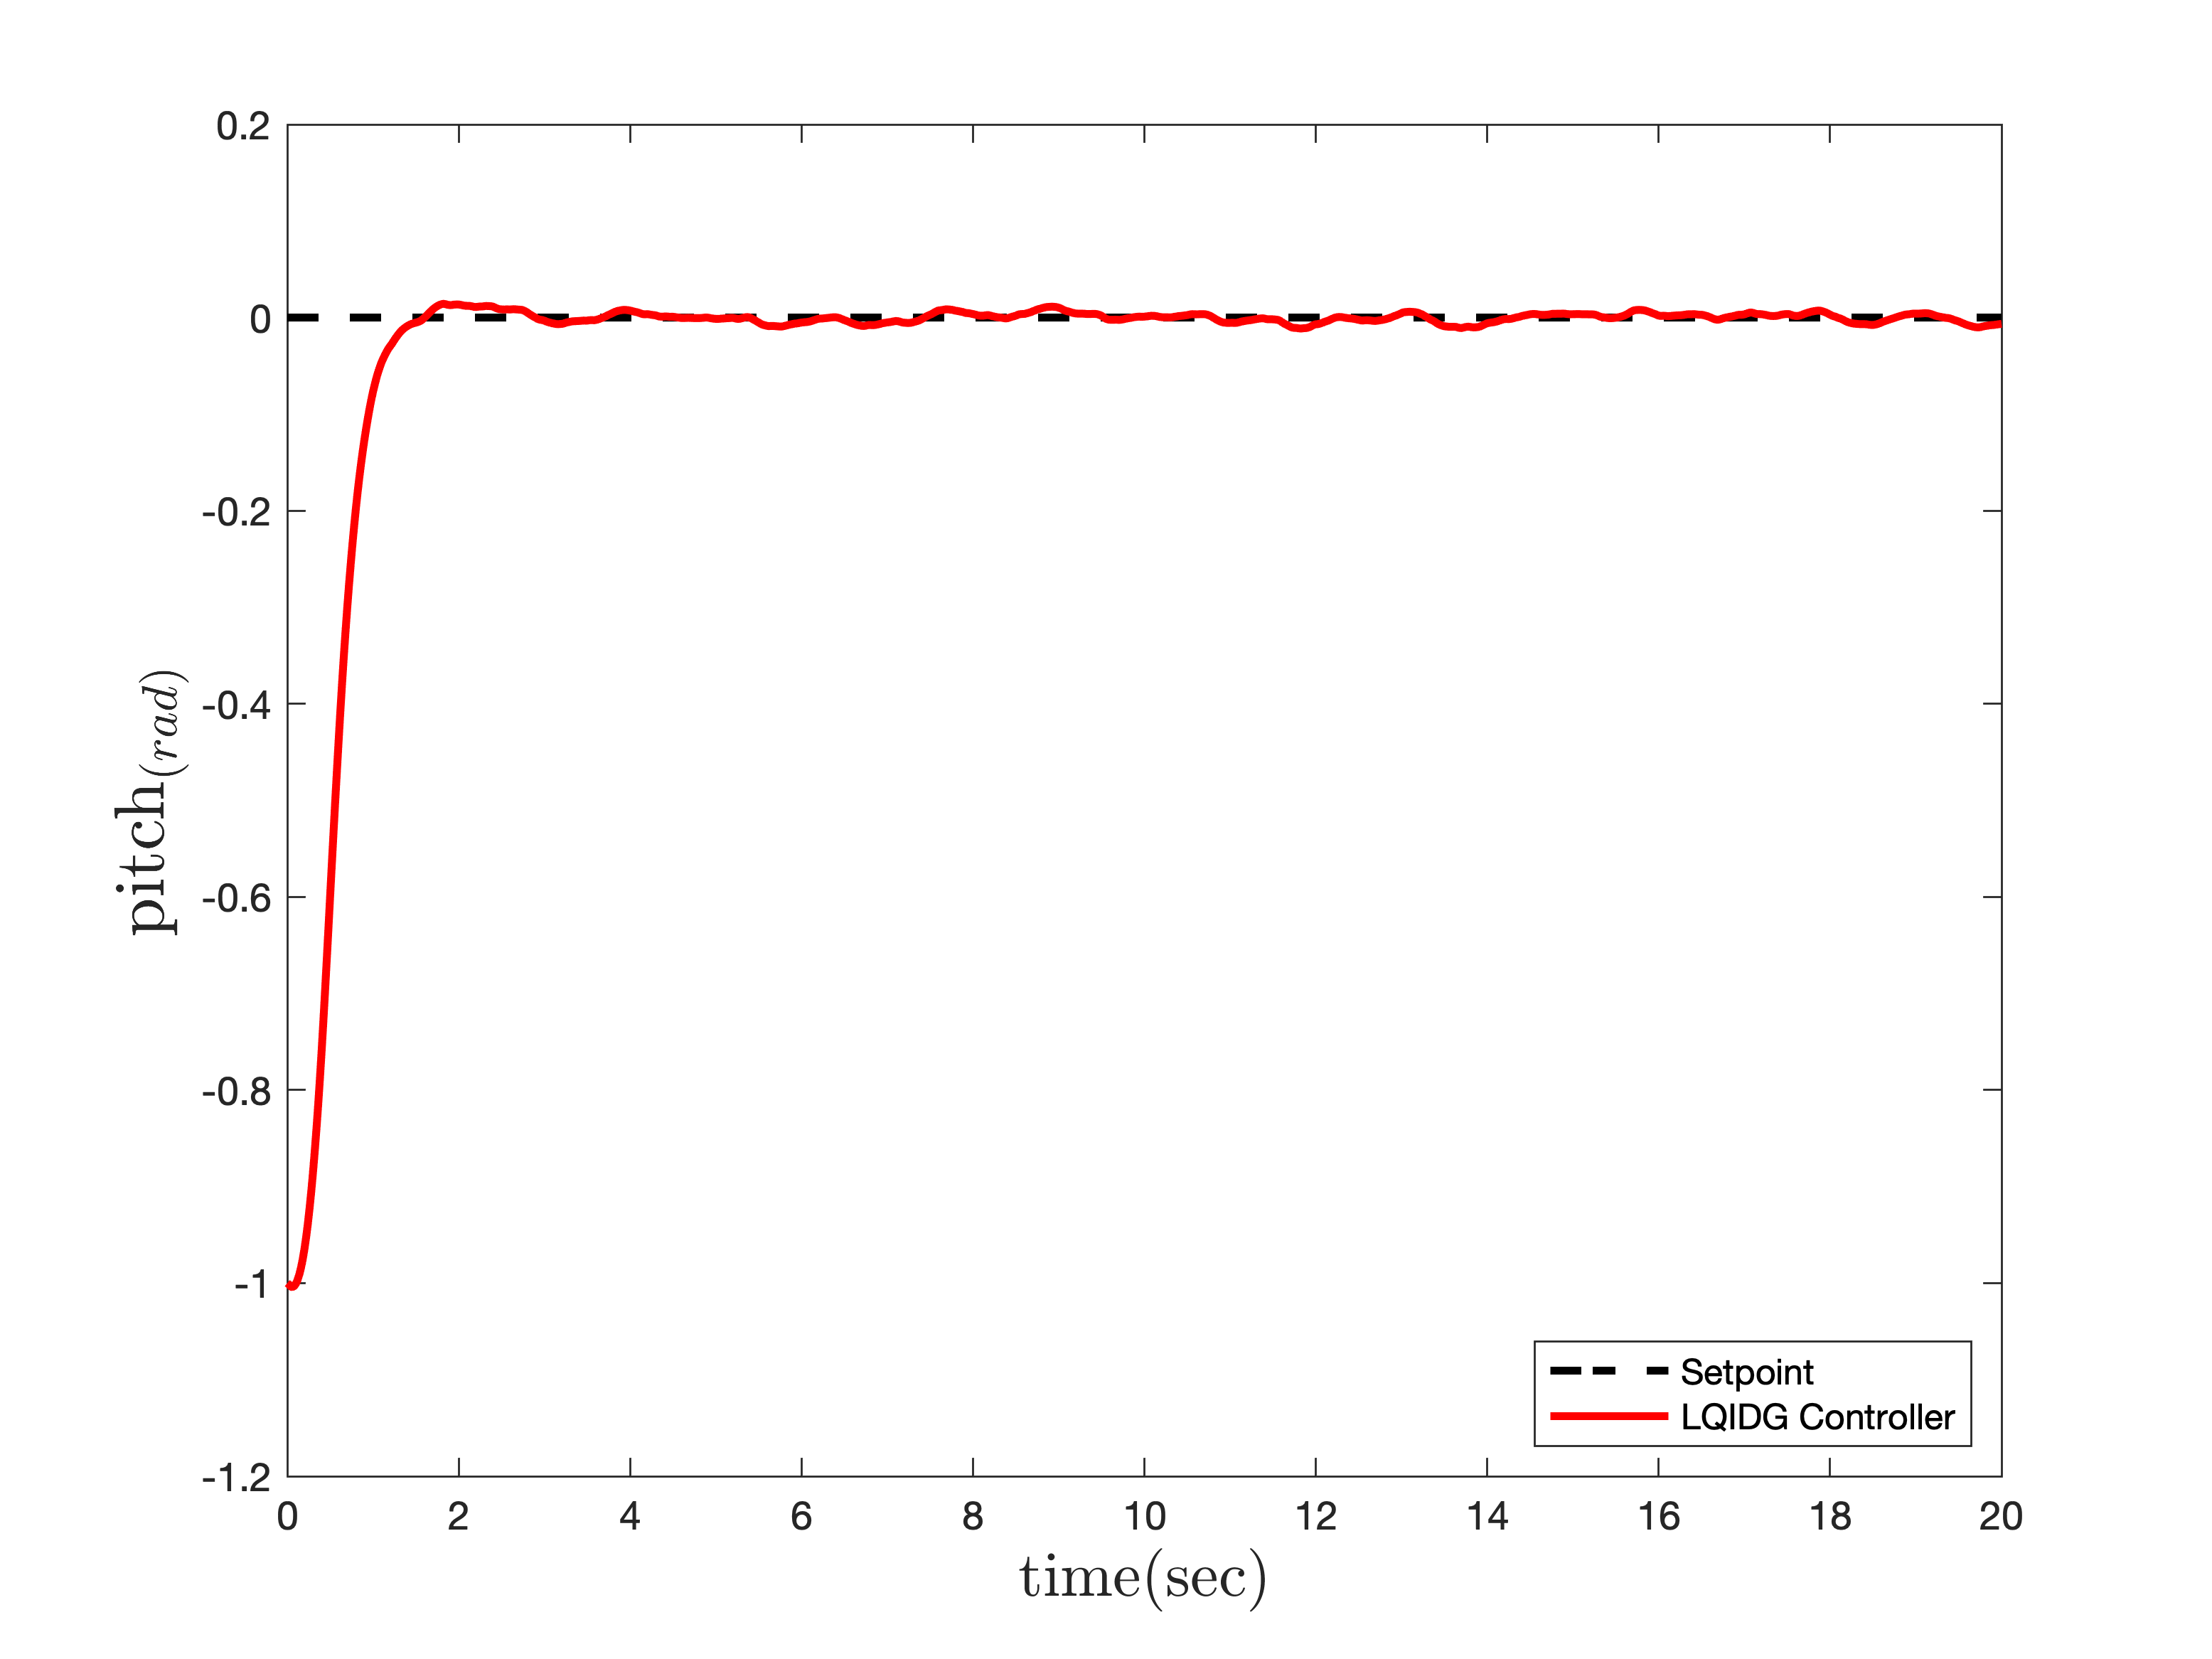
\includegraphics[width=12cm]{../Figures/MIL/LQIDG/Roll_Pitch/lqidg_pitch.png}
%		\caption{تغییرات زاویه پیچ}
%	\end{subfigure}
%	
%\end{figure}
\begin{figure}[H]
	\centering
	\subfigure[تغییرات زاویه رول]{
		\centering
		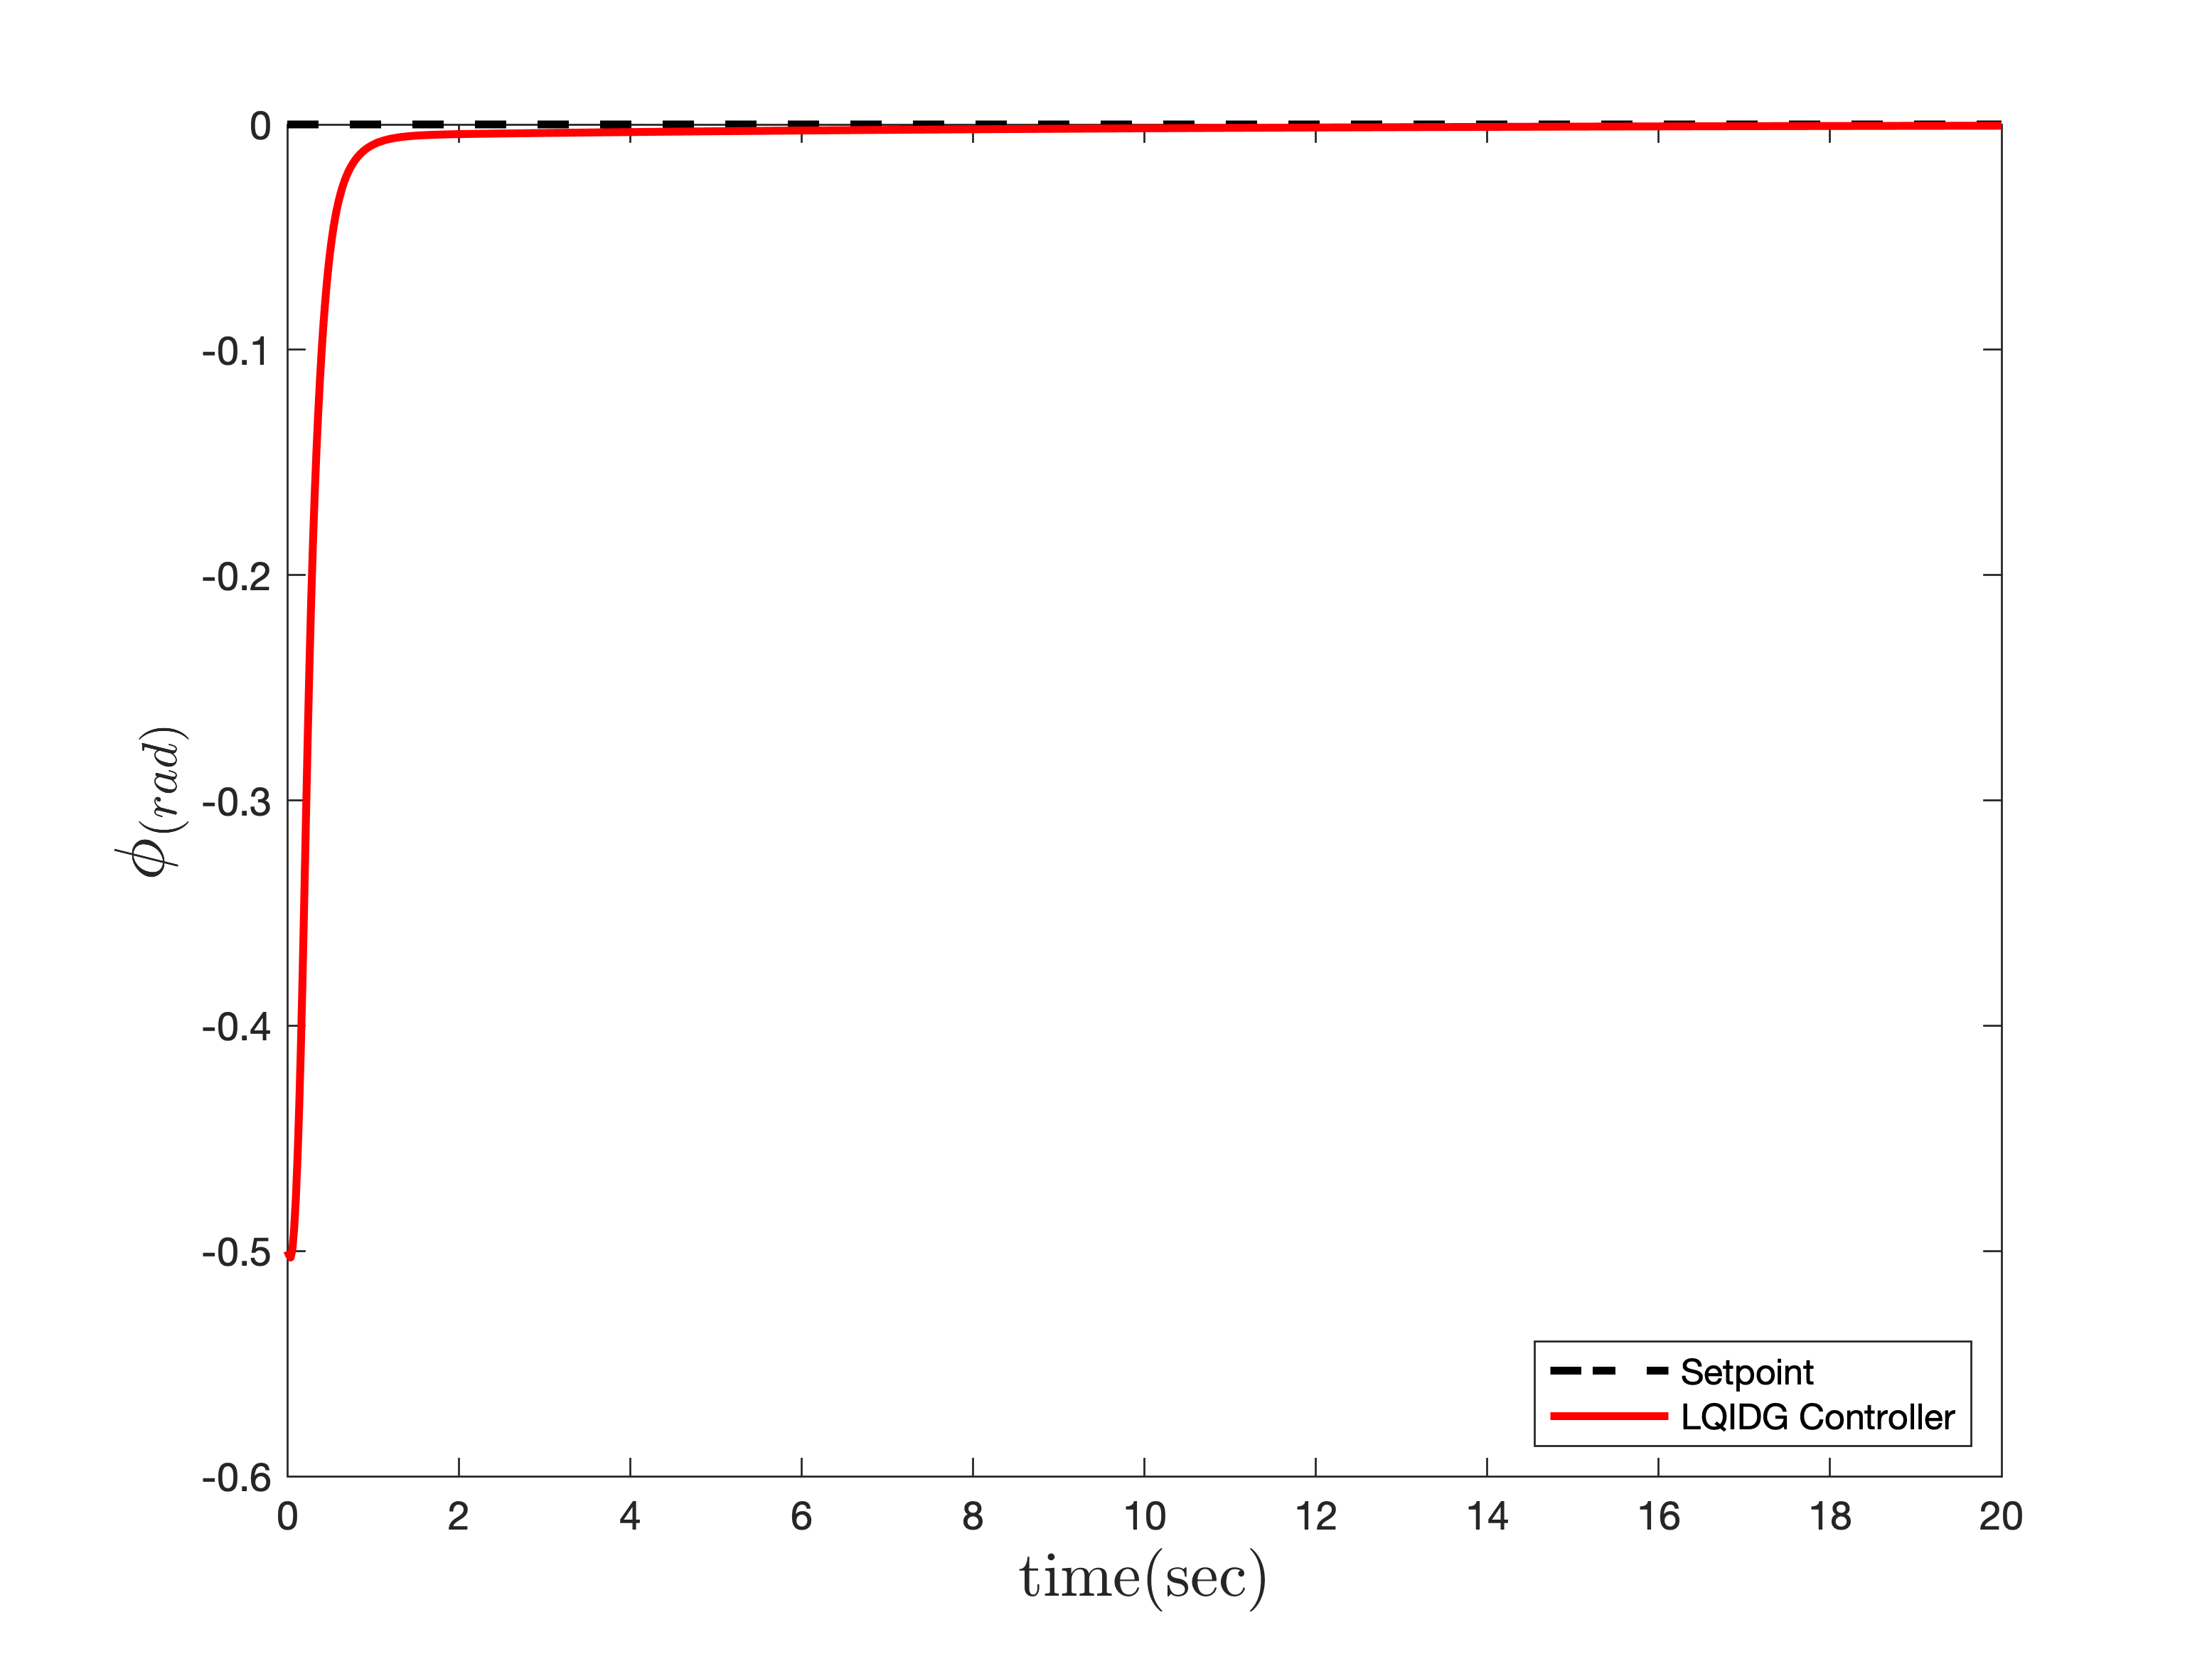
\includegraphics[width=.48\linewidth]{../Figures/MIL/LQIDG/Roll_Pitch/lqidg_roll_nn.png}
	}
	\subfigure[تغییرات زاویه پیچ]{
		\centering
		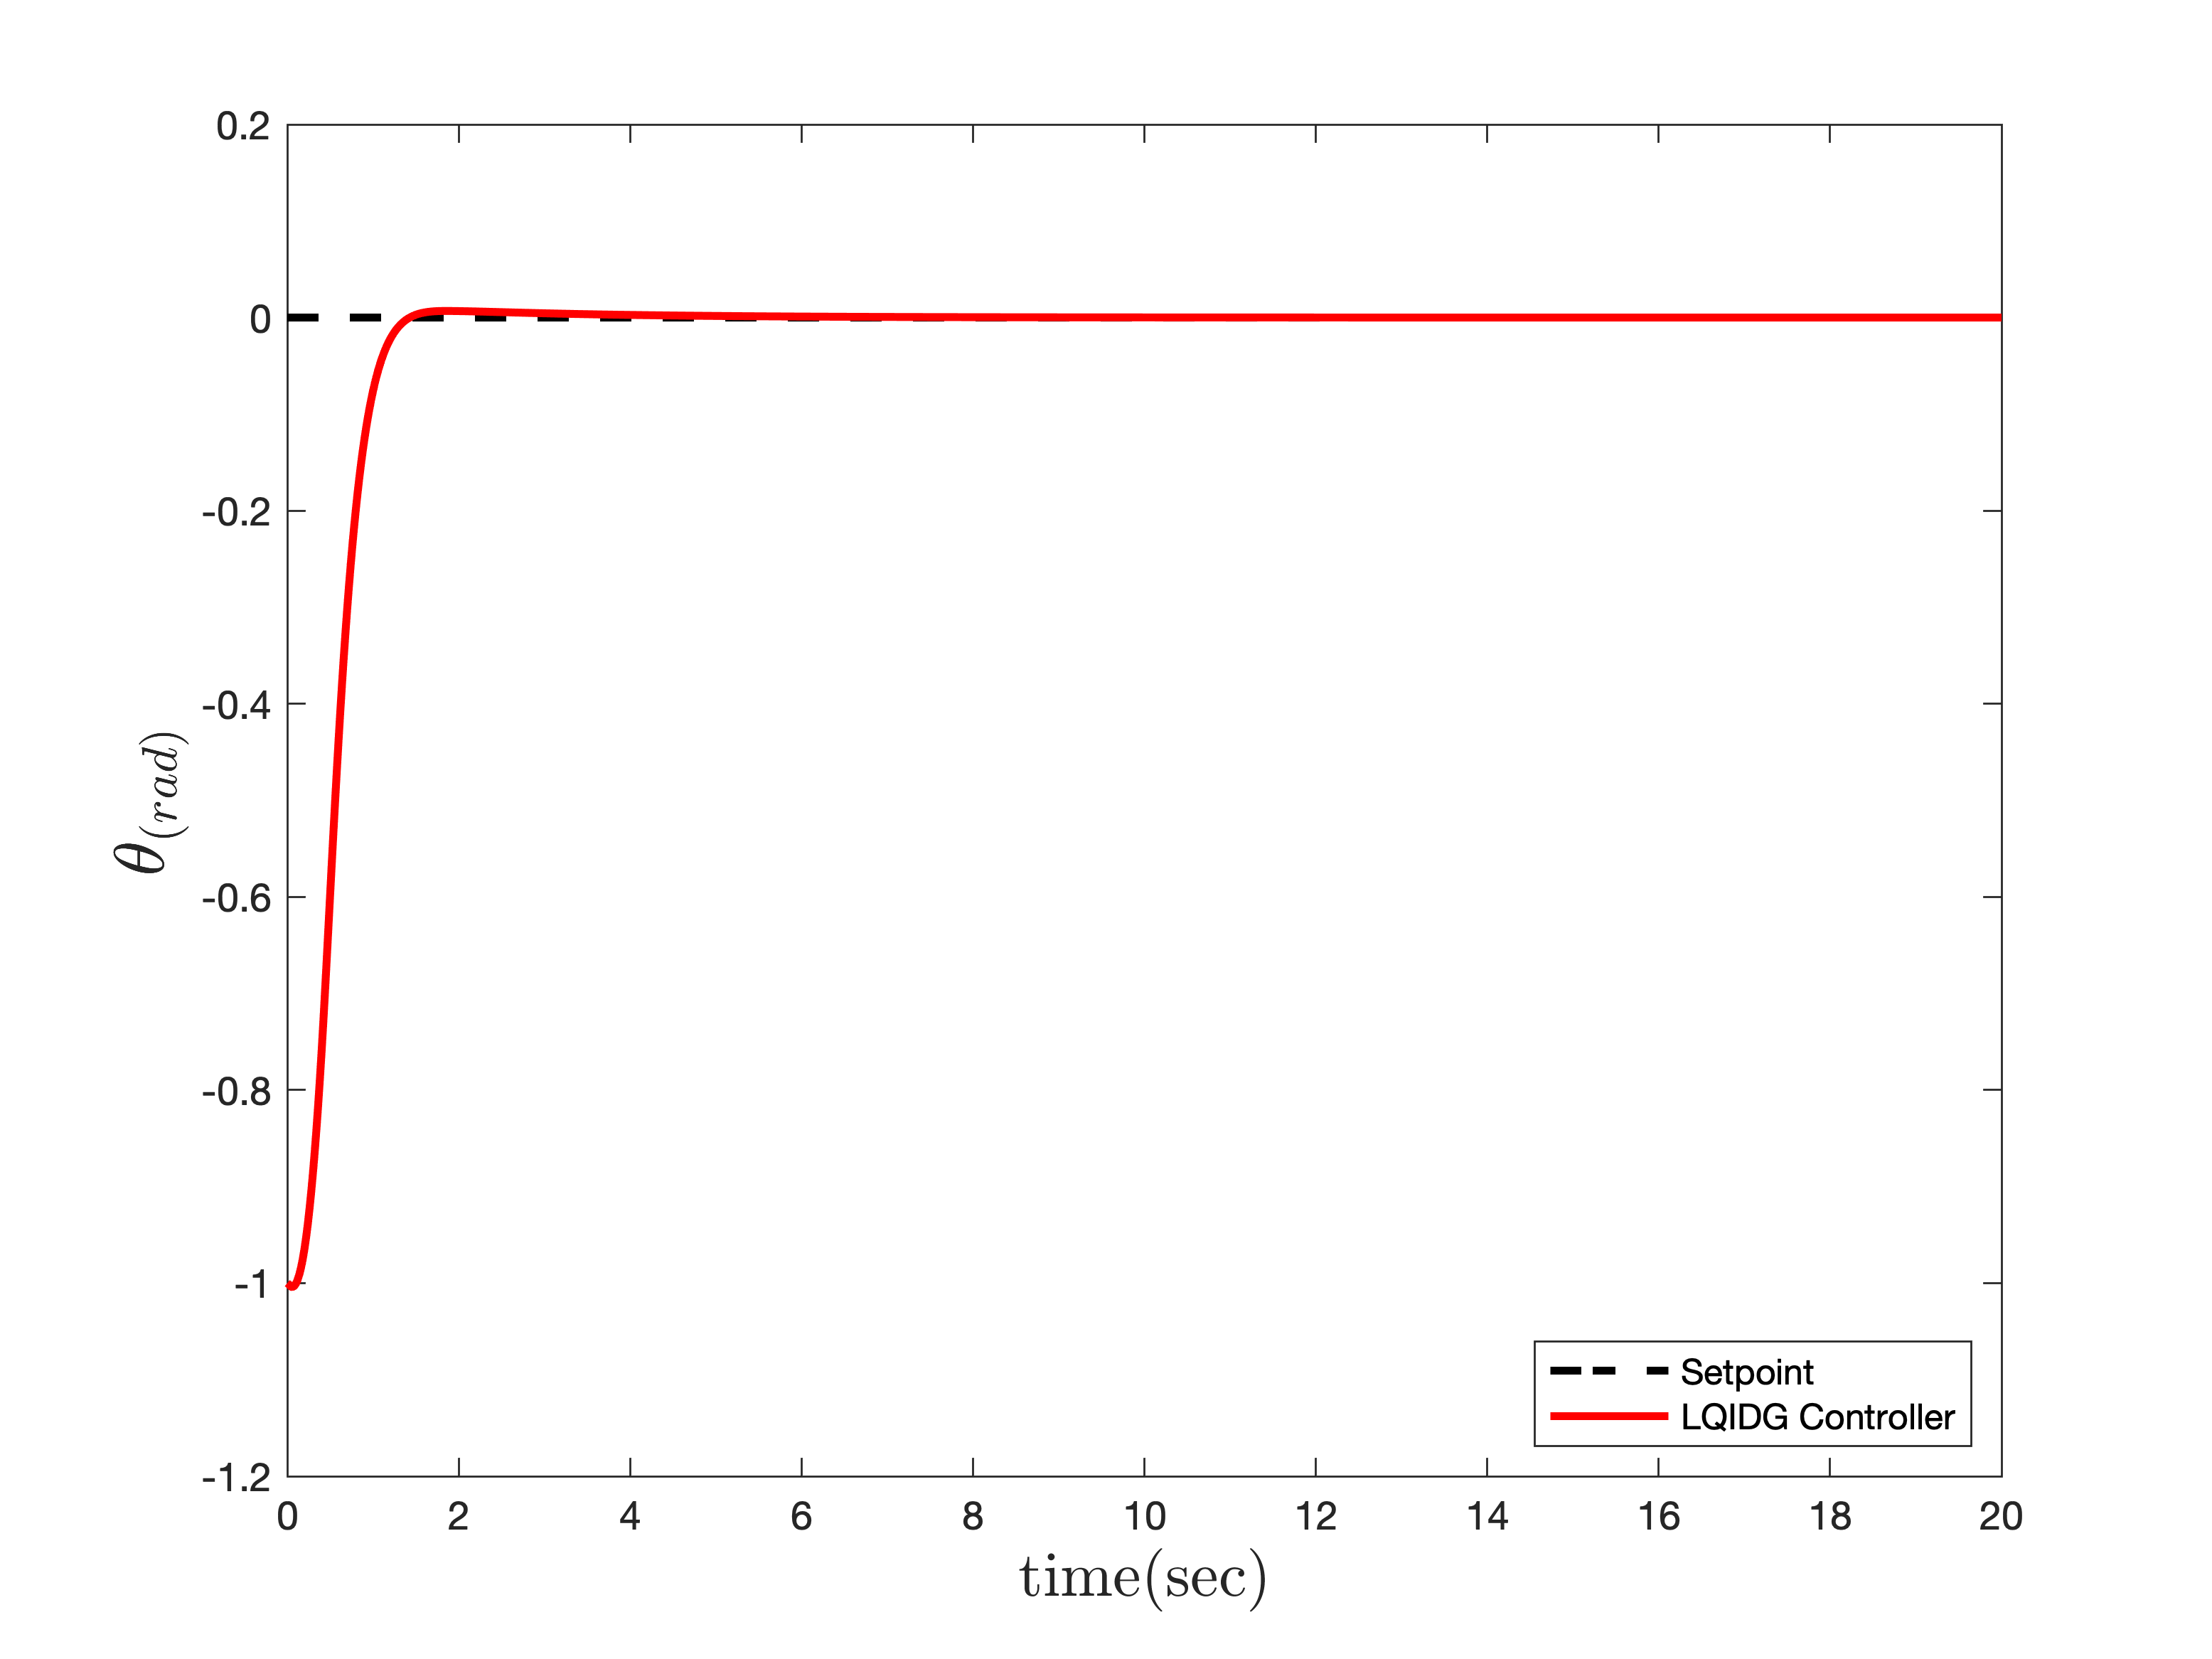
\includegraphics[width=.48\linewidth]{../Figures/MIL/LQIDG/Roll_Pitch/lqidg_pitch_nn.png}
	}
	\caption{‫‪عملکرد کنترل‌کننده \lr{LQIDG} در کنترل زاویه رول و پیچ (تعقیب ورودی صفر)}
	\label{lqidg_roll_pitch_fig_simulation}
\end{figure}



\begin{figure}[H]
	\centering
\subfigure[موتور شماره یک]{
		\centering
		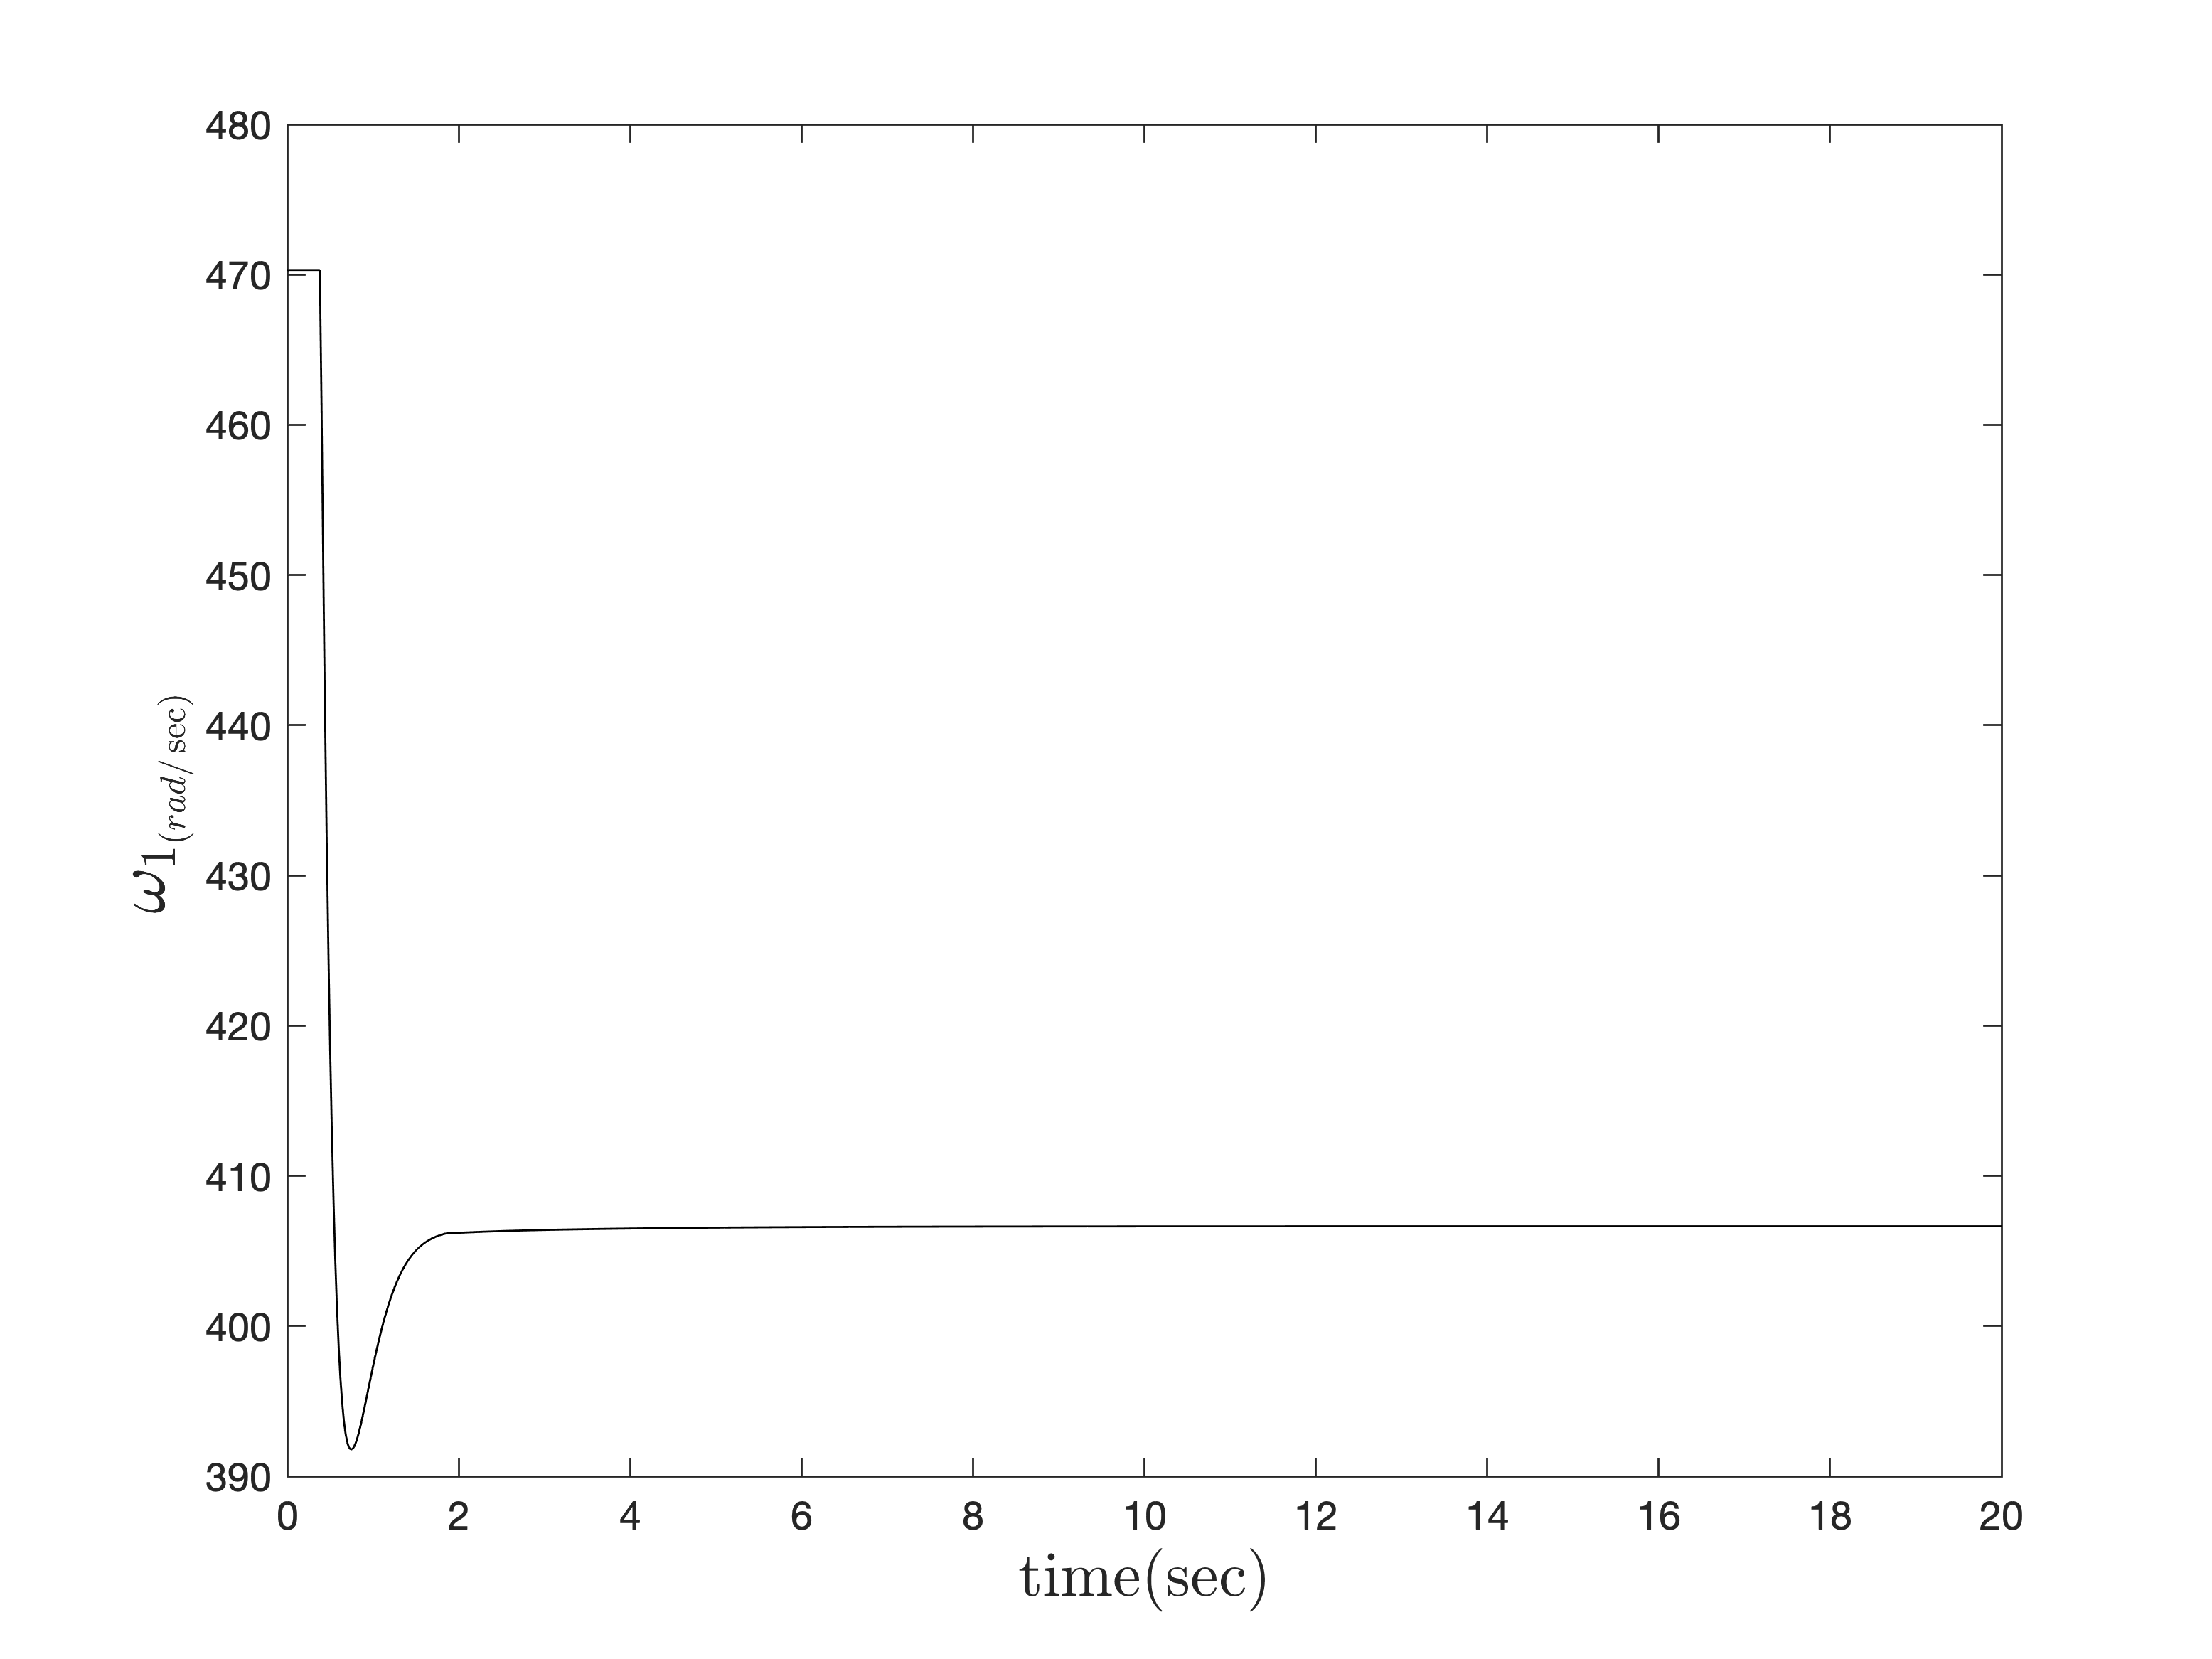
\includegraphics[width=.45\linewidth]{../Figures/MIL/LQIDG/Roll_Pitch/lqidg_roll_pitch_Omega_1_nn.png}
	}
\subfigure[موتور شماره دو]{
	\centering
	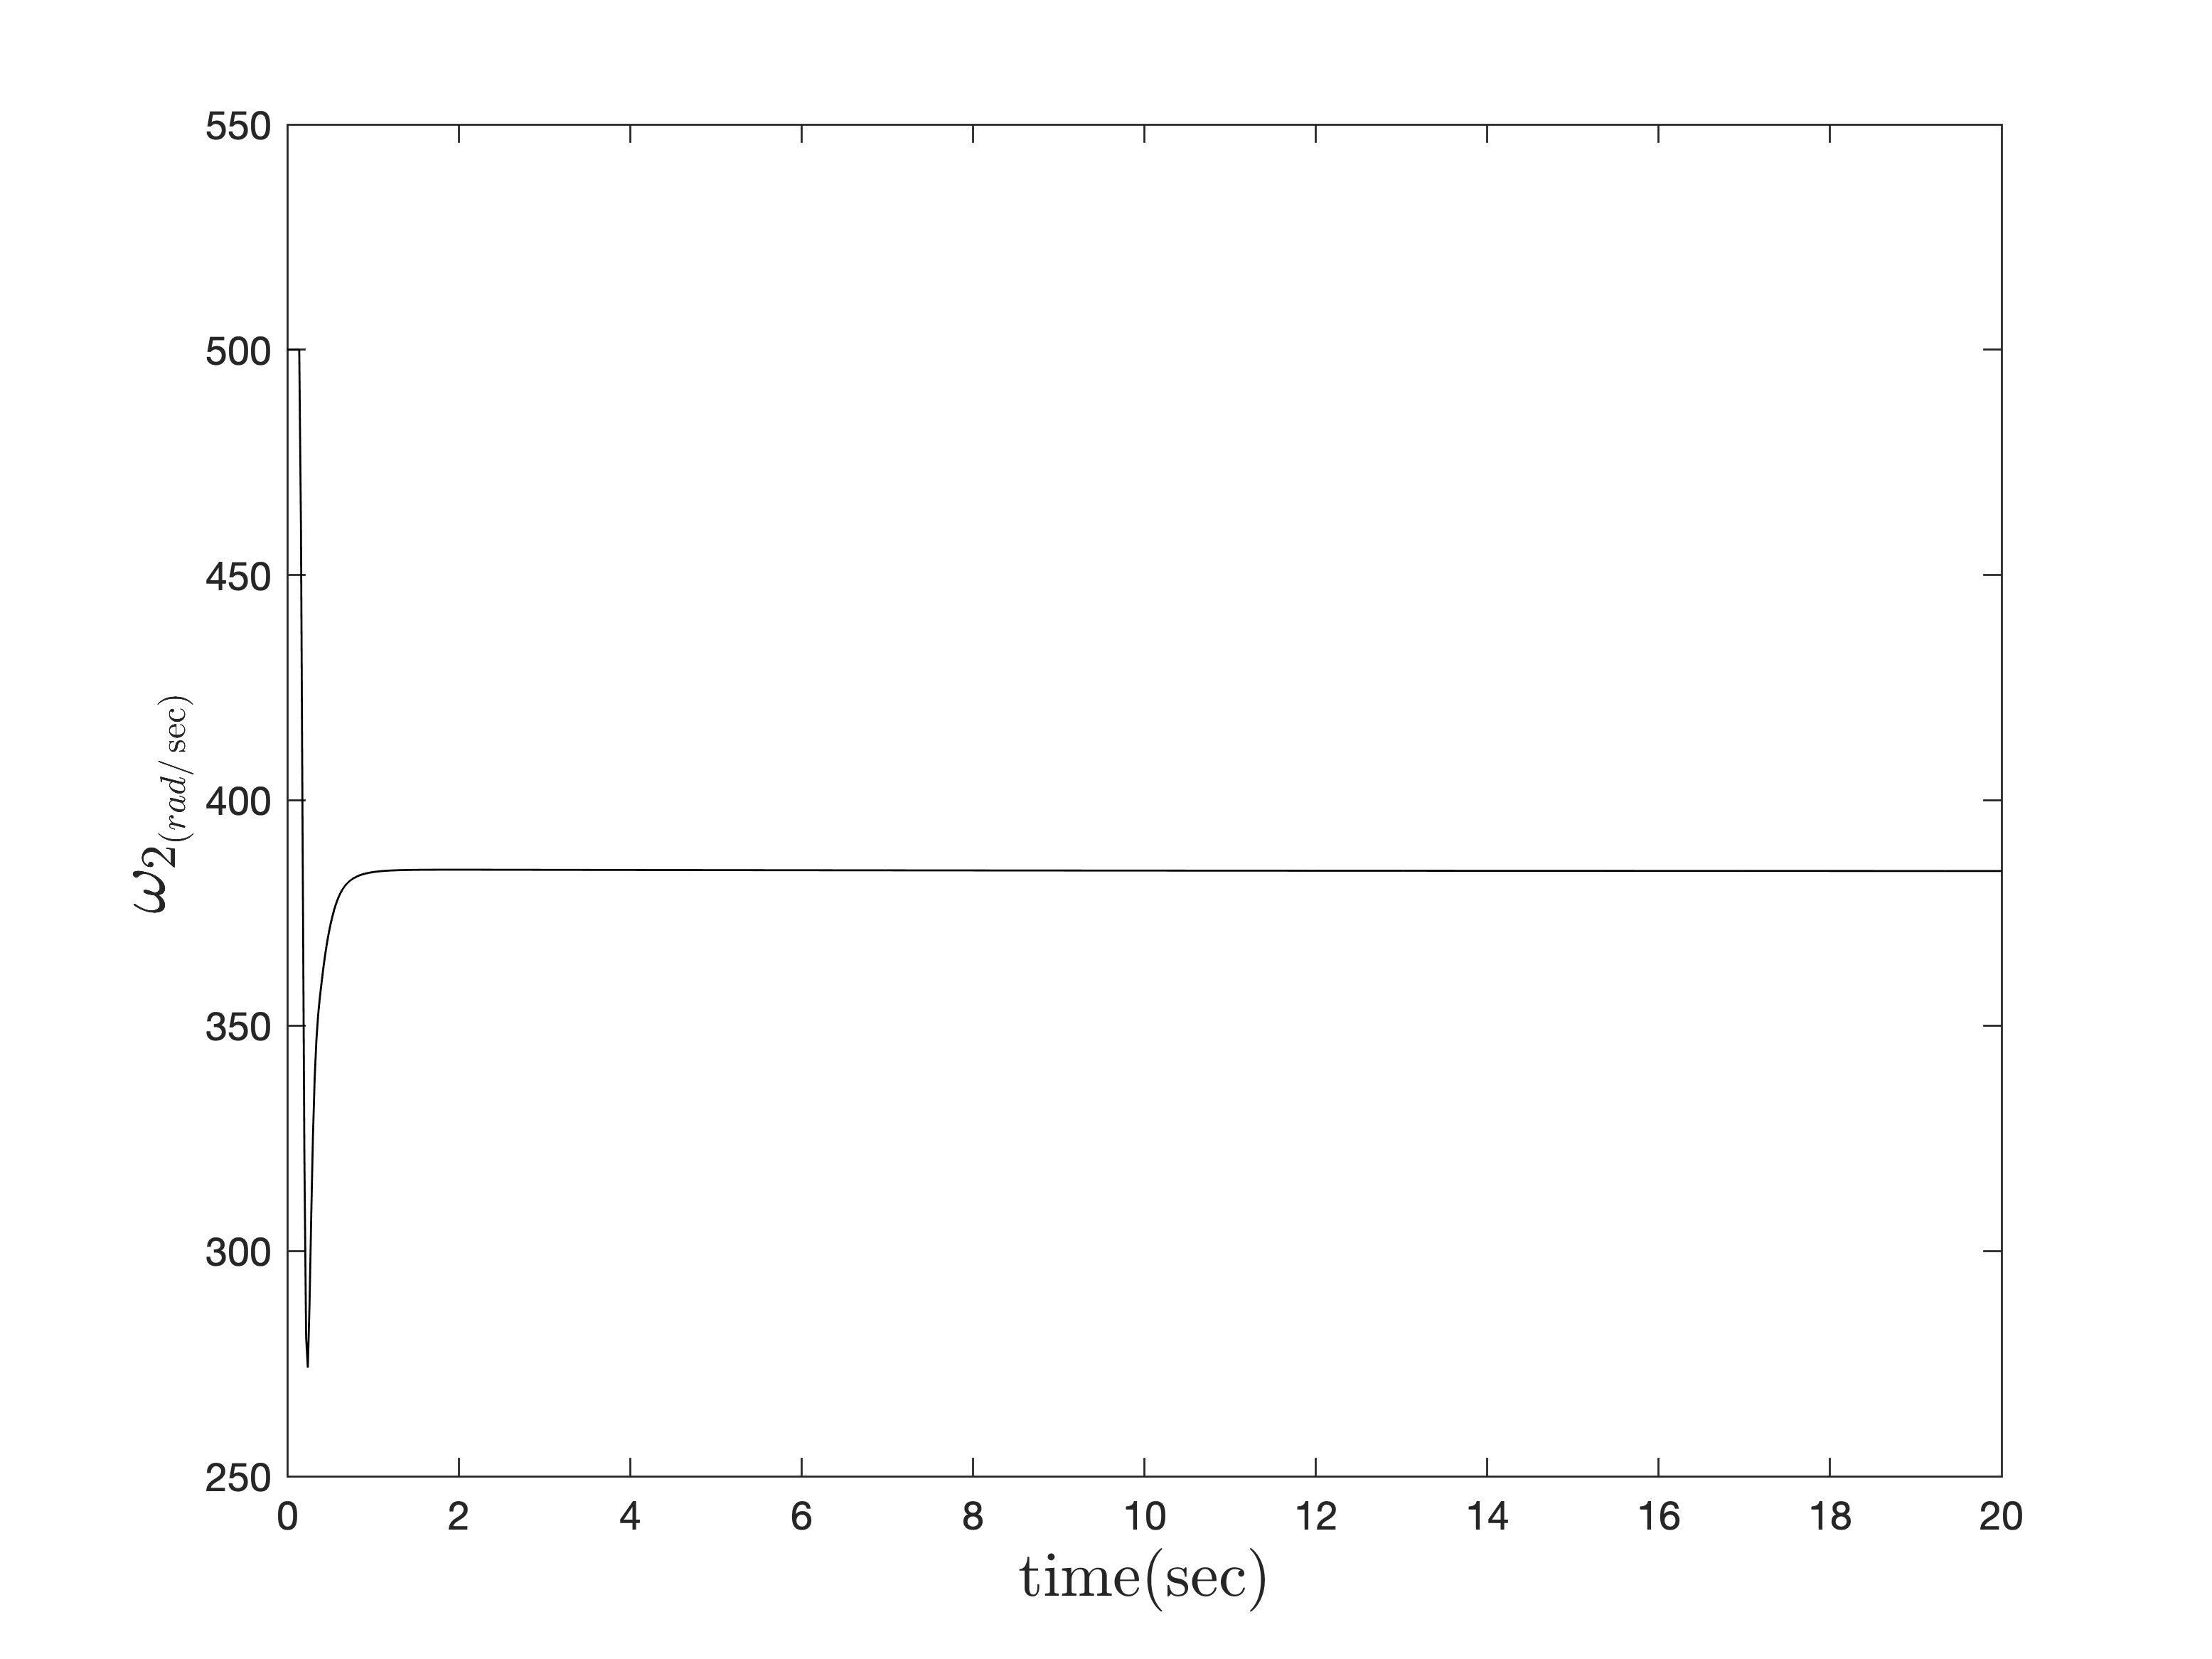
\includegraphics[width=.45\linewidth]{../Figures/MIL/LQIDG/Roll_Pitch/lqidg_roll_pitch_Omega_2_nn.png}
}
\subfigure[موتور شماره سه]{
	\centering
	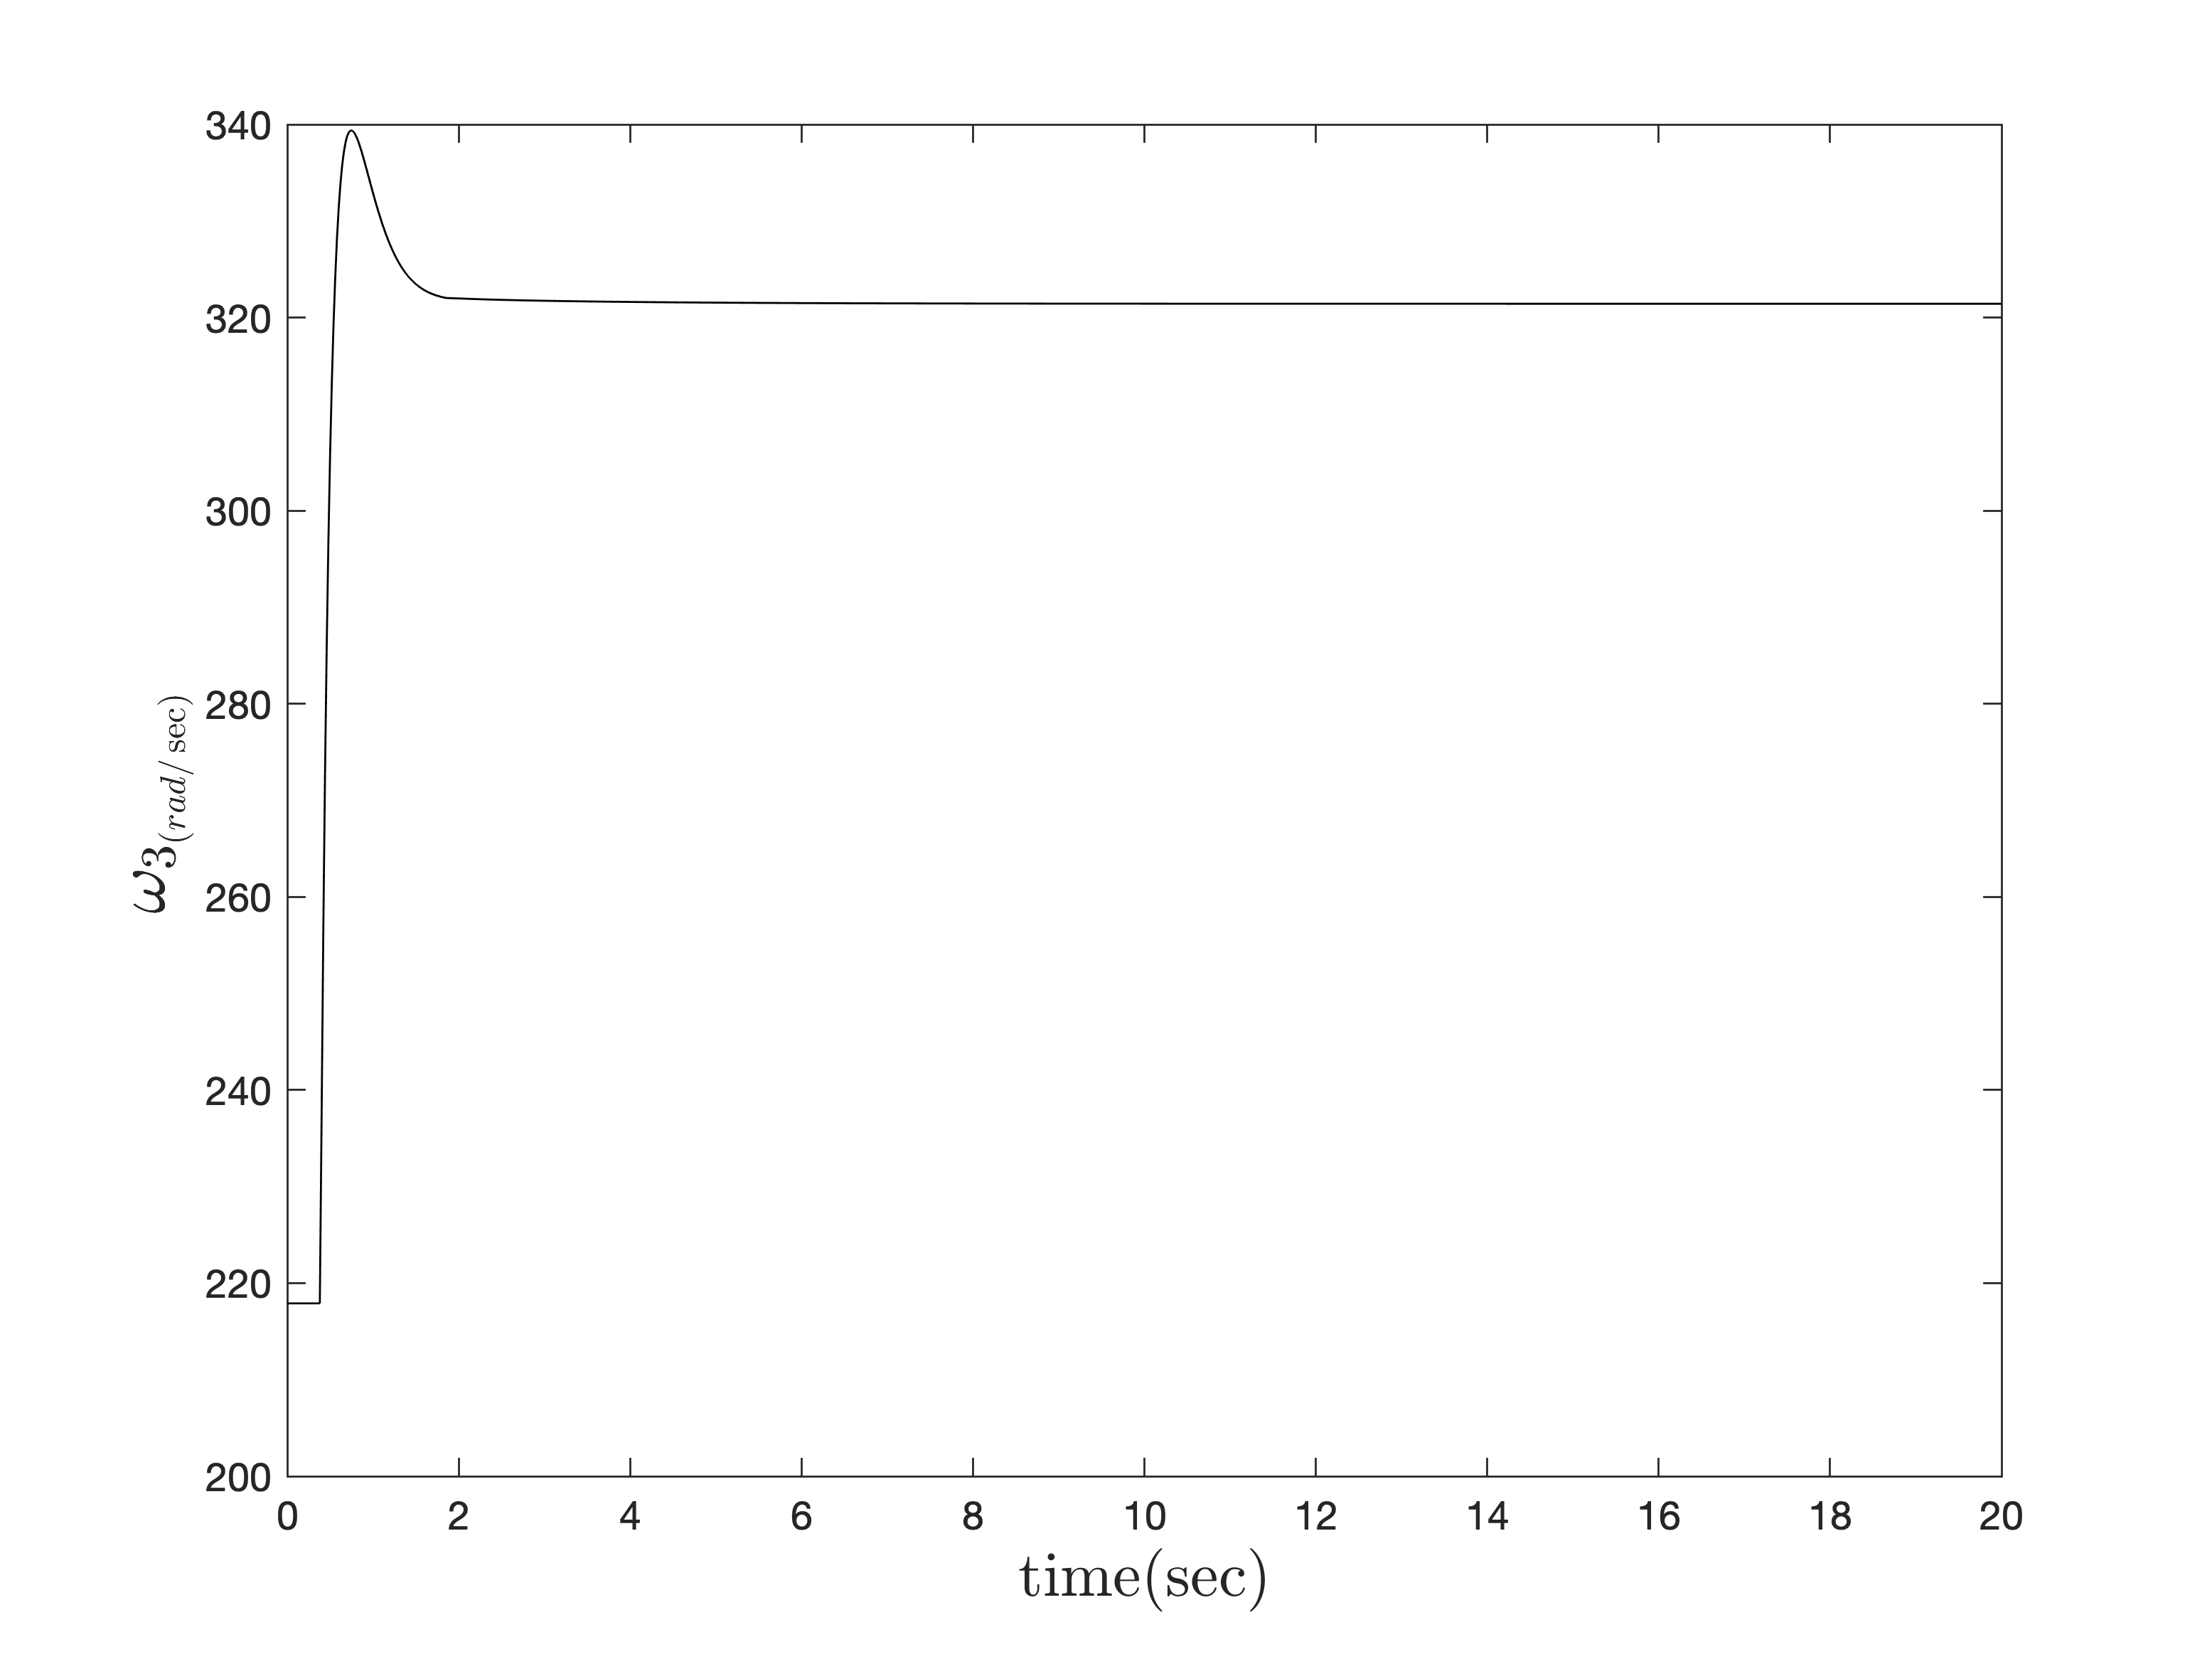
\includegraphics[width=.45\linewidth]{../Figures/MIL/LQIDG/Roll_Pitch/lqidg_roll_pitch_Omega_3_nn.png}
}
\subfigure[موتور شماره چهار]{
	\centering
	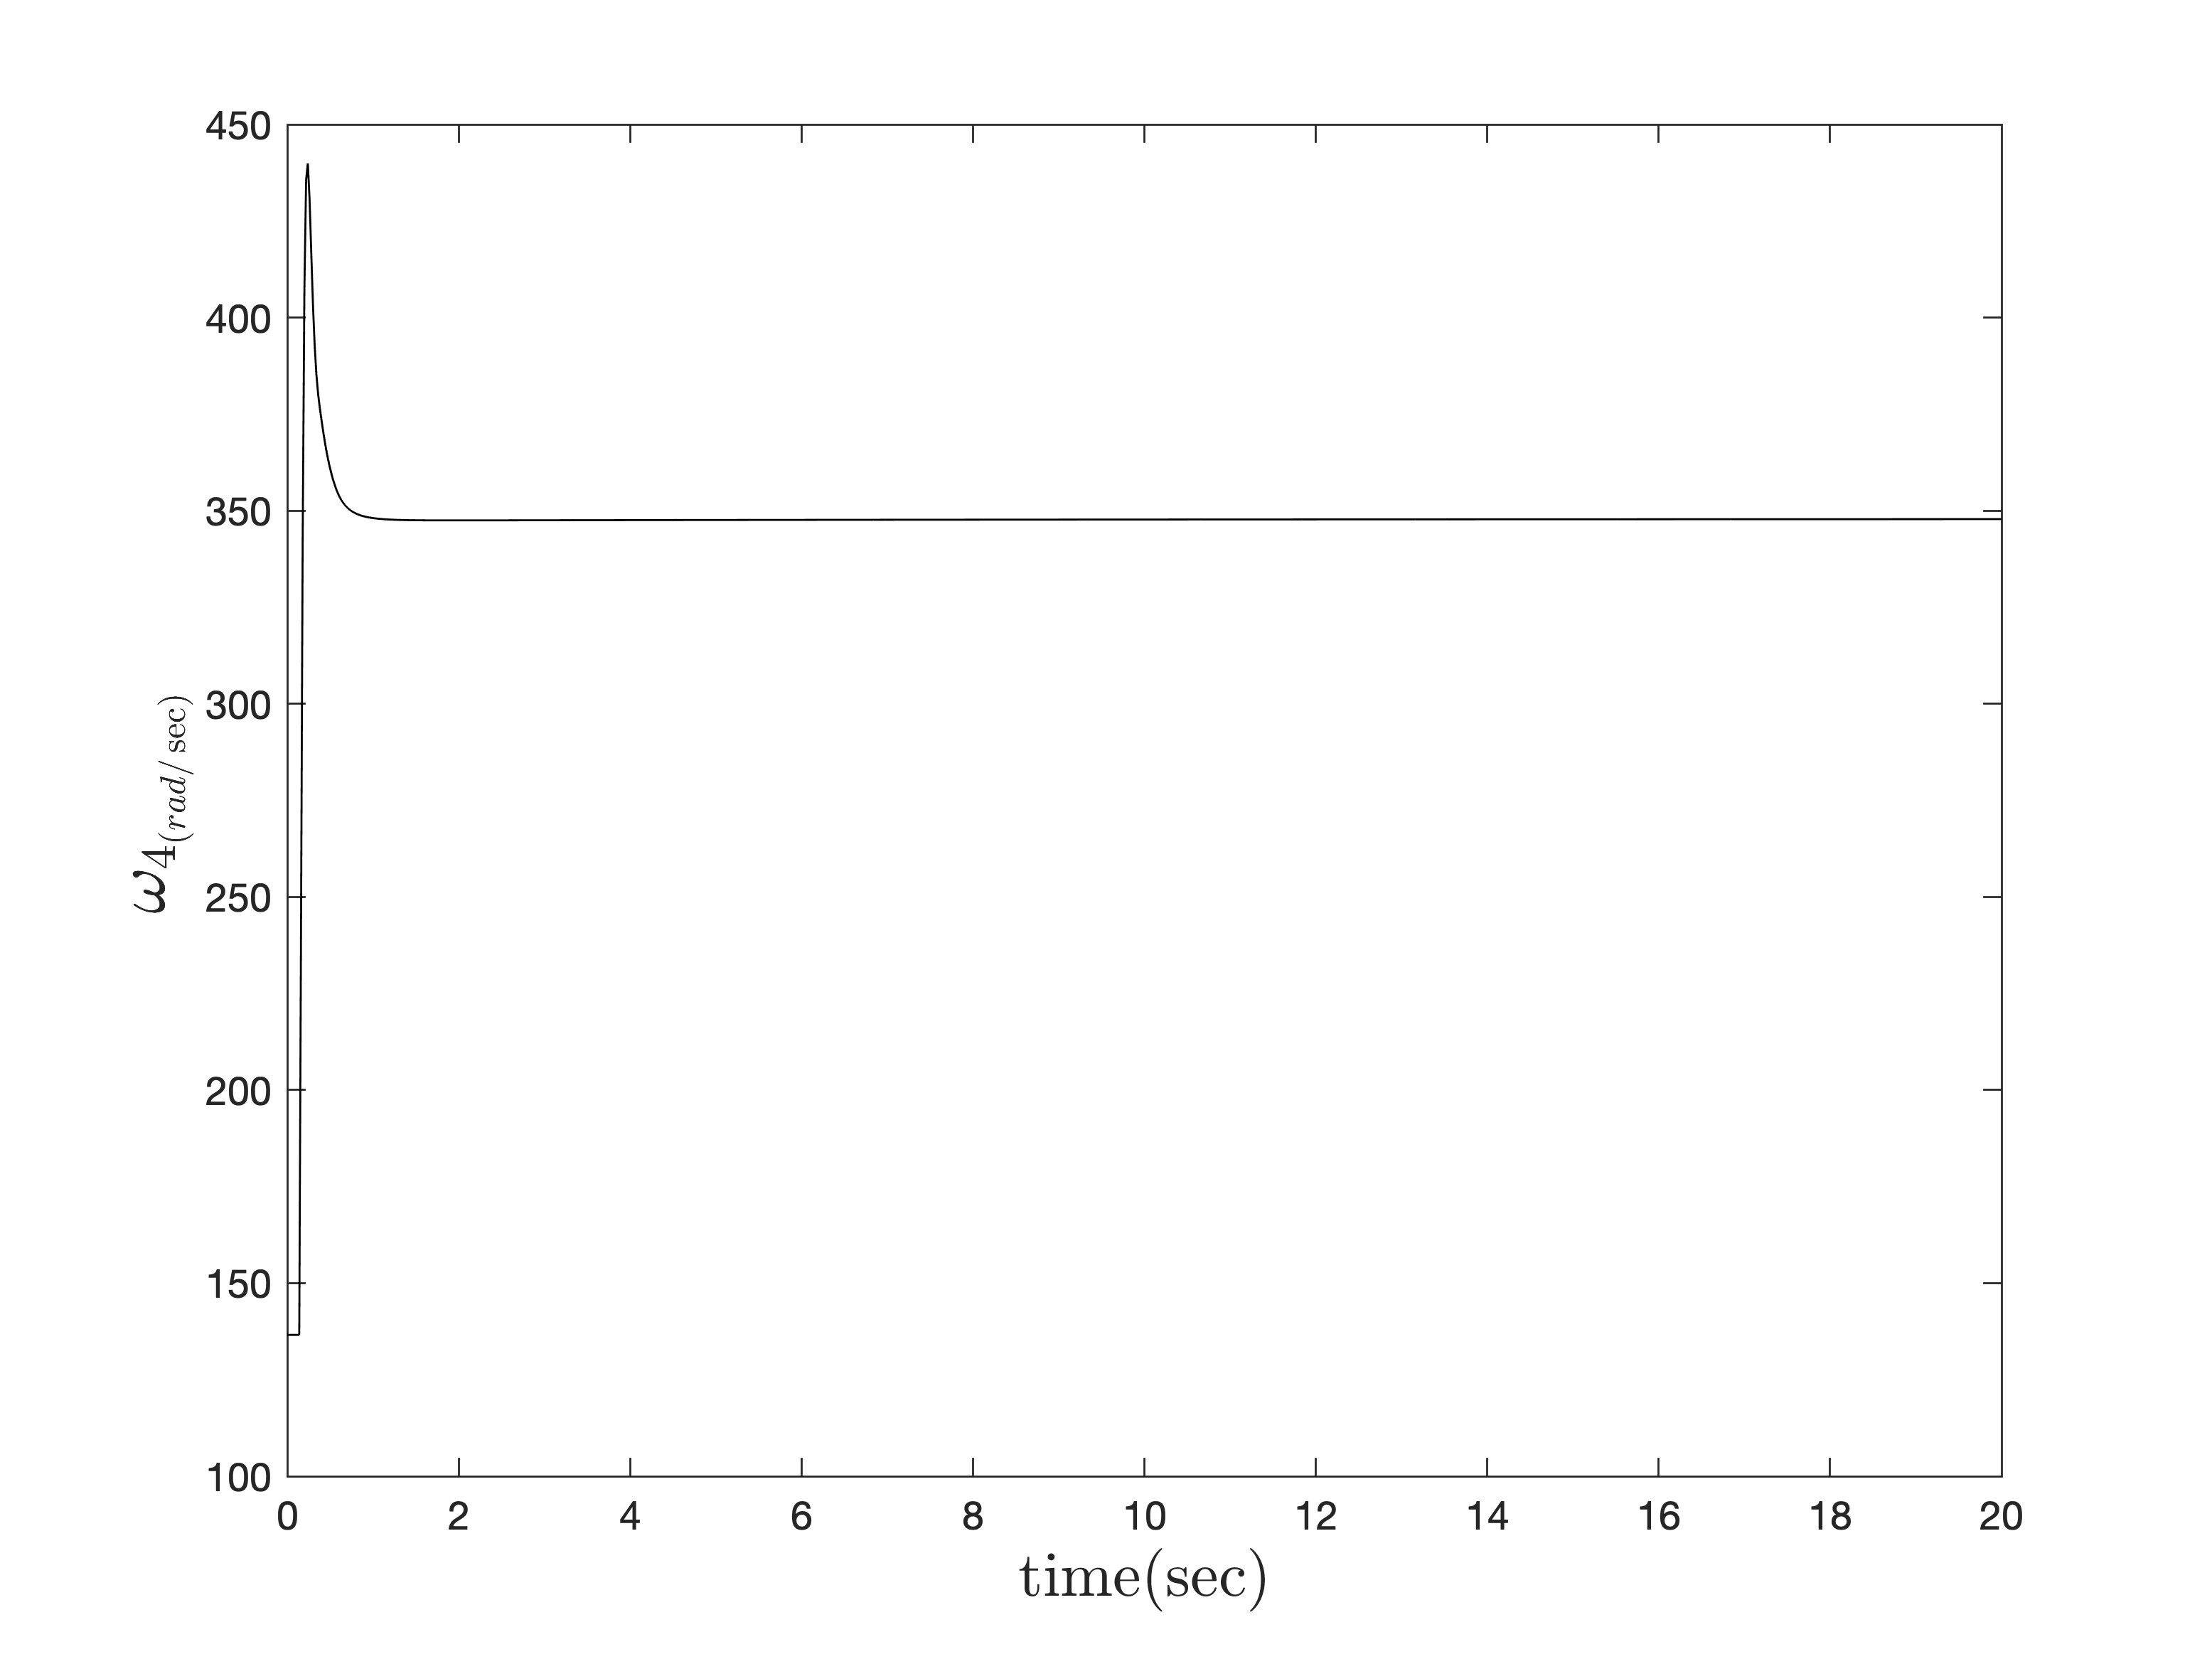
\includegraphics[width=.45\linewidth]{../Figures/MIL/LQIDG/Roll_Pitch/lqidg_roll_pitch_Omega_4_nn.png}
}
	\caption{‫‪فرمان کنترلی موتورها در کنترل زاویه رول و پیچ (تعقیب ورودی صفر)}
\end{figure}


بر اساس خروجی شبیه‌سازی (شکل
\ref{lqidg_roll_pitch_fig_simulation})،
کانال رول در حضور کنترل‌کننده \lr{LQIDG} در حدود پنج ثانیه و کانال پیچ در حدود هشت ثانیه به تعادل می‌رسد و خطای ماندگار آن در حدود صفر است.